\documentclass{article}
\usepackage{amssymb}
\usepackage{color}
\usepackage{listings}
\usepackage{graphicx}


\setlength{\parindent}{1em}
\setlength{\parskip}{1em} % length of the spacing

\lstset{ % General setup for the package
    language=Python,
    basicstyle=\small\sffamily,
    numbers=left,
    numberstyle=\tiny,
    frame=tb,
    tabsize=4,
    columns=fixed,
    showstringspaces=false,
    showtabs=false,
    keepspaces,
    commentstyle=\color{red},
    keywordstyle=\color{blue},
    emphstyle=\ttb\color{deepred},    
    stringstyle=\color{deepgreen}
}

\begin{document}
    \title{Navigation and Intelligent Vehicles, Lab session 1 Report}
    \author{Juan Jose Soriano Escobar}
    \maketitle
    \newpage

    \section*{Disclaimer}

    This lab session is developed with Python Instead of Matlab, due to the lack of experience with Matlab
    and because I am more familiar with Python from the previous courses in the Master program. Additionally,
    Python has several libraries that could be easily use to deploy the solution in a web server or in a embedded system.

    On top of Python, I've used numpy library to manipulate multidimensional array objects, and pylab to display the results in graphs. 

    With all that said, I expect to achieve the same results and learn the same concepts as working with Matlab.

    \section{Simulated measurement data}
    

    As  first, before going into the Kalman Filter application  or coding the model itself, I started by creating the measurements
    as was suggested in the Laboratory document \cite{LabManual}. A normal random distributed noise centered in 0.0 with a standard deviation 0.1, 
    for a constant value of 0.26578 voltages.

    The voltages sampled were simulated for 50 measurements using the fragment of code \ref{lst:measurementData} and illustrated in the figure \ref{fig:data}.

    \begin{lstlisting}[language=Python, caption= Measurement data simulation, label={lst:measurementData}]
        import numpy as np

        # for 50 measurements simulated
        iterations = 50

        x = np.full(iterations, 0.26578)
        noise = np.random.normal(0.0, 0.1, iterations) 
        Z = x + noise
    \end{lstlisting}
    
    \begin{figure}
        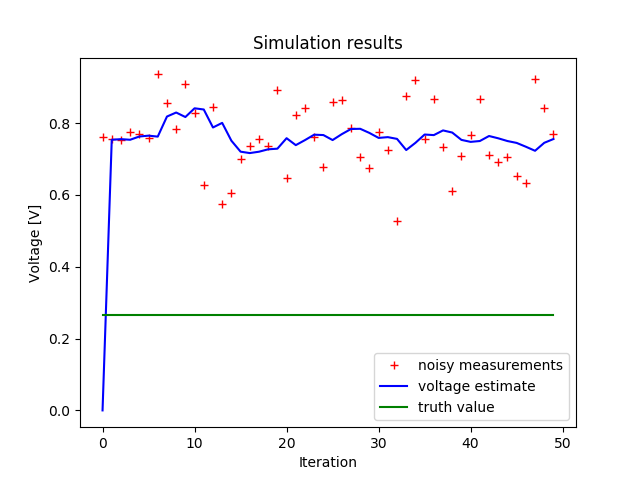
\includegraphics{./img/nc_.png}
        \caption{Simulated measurements.}
        \label{fig:data}
    \end{figure}
      

    \section{Programing the Kalman Filter}

    Following the Kalman Filter logic from the theory, the code is divided in two functions. The first one is the  prediction function for the
    future value of the state value and the error covariance. The function developed for the predictions is presented in the section of code [2]

    **code**

    \begin{equation}
        x = x + 1
    \end{equation}

    The prediction function predict the values of the state value and the error covariance receiving 5 arguments:

    X: The state estimate of the previous step.
    P: The state covariance of the previous step.
    A: The transition matrix.
    Q: The process noise covariance matrix.
    B: The input effect matrix.
    U: The control input.

    With those arguments the new X and P are predicted based on the reviewed formulas [1] [2].

    Once the prediction is done, it is necessary to update the measurement and verify the error prediction based on the real measured value.
    In this order, the update functions presented in the section [5], receives 6 arguments:

    X: The state estimate.
    P: The state covariance.
    C: The measurement matrix.
    K: The gain or blending value (Kalman gain matrix).
    Z: The measurement.
    R: The measurement covariance matrix.

    To compute the residuals and calculate the gain or blending value K, together with the updated value of the state estimate X and the
    state covariance P. 

    The calculations done in the update function are based on the equation [1]. Where MP is the measurement prediction, 'MPC' is the measurement
    prediction covariance and residual is the difference between the measured and predicted value.

    \newpage

    This two functions are enough to apply the Kalman Filter to the specific case of study. Thereafter, a for loop is needed to simulated the
    50 iterations, where the function and update value are going to be implemented as is shown in the section [6].

    **insert section**

    At this point, the code is ready to be applied in the the voltage measurement problem.

    \section{Code implemention}
        
    As always in any algorithm or code  to be executed, the first step is to declare the variables with it initial values (see fig [x]).

    A = 1 - The state is a constant
    U = 0 - There is no control input
    B = 0 - There is no control input
    C = 1 - The noisy measurement is direct
    Q = 10e-5 - Process variance
    R = 0.01 - given from the problem as a constant noise
    X = np.zeros(iterations)  - Initializing voltage estimate the array with the number of iterations 
    P = np.zeros(iterations) - Initializing error estimate the array with the number of iterations
    K = np.zeros(iterations) - gain or blending factor initialization
    ISE = np.zeros(iterations) - Instant Square Error
    MSE = np.zeros(iterations) - Mean Square Error
    x = np.full(iterations, 0.26578)
    noise = np.random.normal(0.0, 0.1, iterations) - for 50 measurements simulated
    Z = x + noise

    initial state and error covariance values
    X[0] = 0.0
    P[0] = 1.0

    There we define from the given problem, a Process variance Q of 10e-5, a constant noise R of 0.01 and a measure matrix C=1.

    Results

    Q = 10e-5 and R = 0.01

    Q = 10e-5 and R = 0.00001 (R increased on a factor of 1000)

    Q = 10e-5 and R = 10 (R decreased on a factor of 1000)

    Q = 10e-8 and R = 0.01 (Q increased on a factor of 1000)

    Q = 10e-2 and R = 0.01 (Q decreased on a factor of 1000)

   

    \bibliography{report}
    \bibliographystyle{ieeetr}

    lab document
    % http://biorobotics.ri.cmu.edu/papers/sbp_papers/integrated3/kleeman_kalman_basics.pdf
    % https://www.cl.cam.ac.uk/~rmf25/papers/Understanding%20the%20Basis%20of%20the%20Kalman%20Filter.pdf
    % Implementation of Kalman Filter with Python Language ... pdf
    % http://scottlobdell.me/2014/08/kalman-filtering-python-reading-sensor-input/

\end{document}
